%===================================== CHAP 3 =================================

\chapter{Research Method}\label{chap:3}

\iffalse
The developed application is at heart a mean to answer our main research question; How can intelligent recommendation increase student' motivation for studying abroad? And what information and features are important for an IS to be used? This chapter elaborates on the methods and data collection used to collect data to answer the research questions.

Using methods proven to be influential and working is essential for this project. The project does not develop any new methods but takes use of others that are well known in the research community. Such as quantitative data gathering through surveys.The methods introduced in this chapter give descriptions on how the data was gathered and the different experiments performed.

\section{Survey and questionnaires}

The surveys will be conducted through online service providers that provide the framework for the survey. The answer to the survey will then be stored in an datasheet to be analysed at a later point. Some survey sites also includes simple data analysis that give more information on the data collected in a survey.

Measuring the quality of the project as a whole will be done by analysing several factors of the research and development. We will in the project analyse the qualitative data resulting from interviews and surveys on both the manifest level and latent level of analysis. This will give a better understanding on both the clear results and what we can infer or imply from the questions.

We can use the qualitative content analysis methods presented by S. Elo and H. Kyngäs\cite{elo2008qualitative} for systematic, rule-guided qualitative text analysis in the interview and survey questions. This model will help preserve the advantages of quantitative analysis in the qualitative based research results. The steps for the content analysis is described in figure\ref{qualitytative_content}. 

The research in information systems varies to other fields by having a more practical approach to the research. The results are often given using empirical methods on users by doing usability testing and surveys. Knowing how to do perform the analysis in a correct way is important both for the quality of the results and the research validity. A book on empirical research methods have identified the common pitfalls and describes how to avoid them \cite{kitchenham2002preliminary}.

There is several relevant books and literature on analysis that should be read before starting evaluating the project. One of these include “Qualitative evaluation and research methods” by M. Q. Patton [4]. This book introduces method for analysis and evaluation that might prove useful in the project.

\begin{figure}
    \centering
    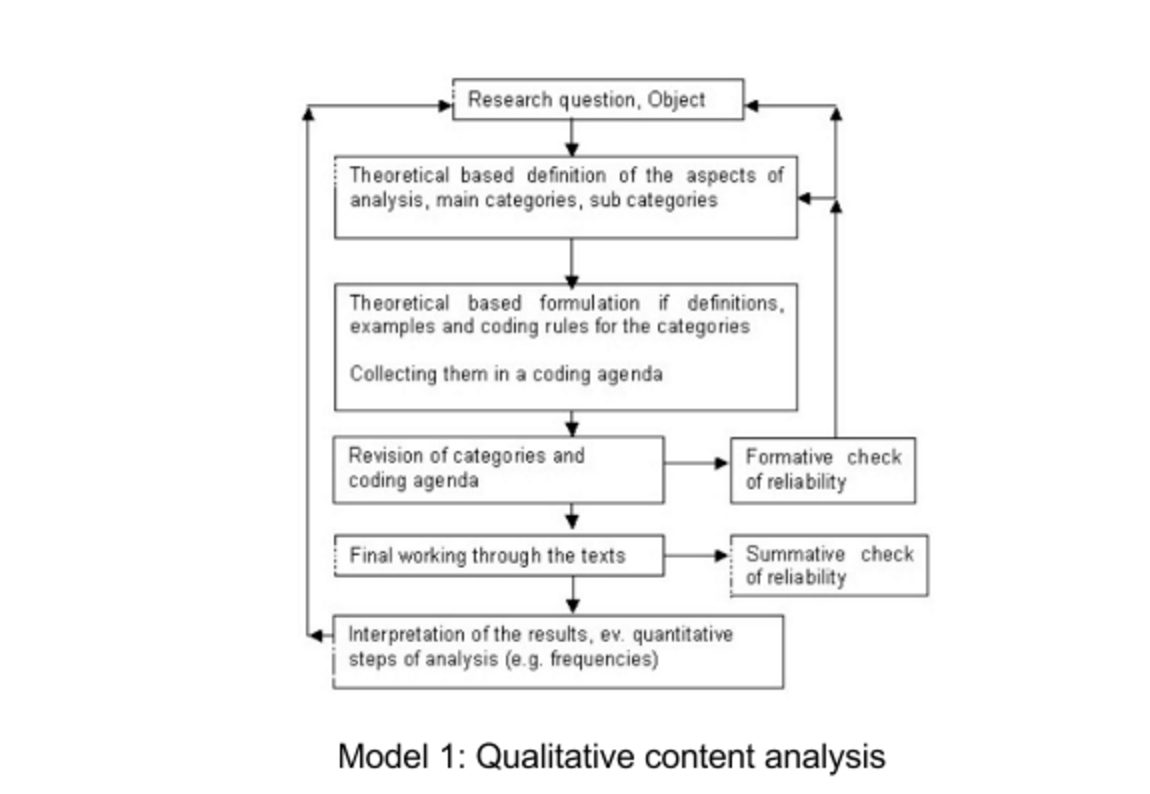
\includegraphics[width=\textwidth]{fig/method.png}
    \label{fig:qualitytative_content}
    \caption{The outlined research process\cite{oates2005researching}}
\end{figure}

\section{Development and prototyping}

\subsection{Iterative design process}
The development of the systems will be done in an iterative process to be able to quickly adapt to user feedback and changes. This will also allow constant change and tweaking of similarity functions and their weighting to better provide a relevant result.

\subsection{Development methodologies}


\section{Observation and experiments}


\subsection{Usability testing}
Usability testing will be performed during the project to evaluate system design and relevance. We will follow the guide *** to usability testing. The project will have different phases of usability testing that focus on different aspects of the system. According to *** this improves ****...???. 

\subsection{Testing Utsida on Students}
The main motivation for the research project is to make the activity of finding a university, as well as what kind of subjects is reasonable to take for a student. Because the current system used at NTNU is mainly performed manually, the process is not very seamless and straightforward. Therefore, testing this system on students throughout its development is very important.

\fi






Using Oates'\cite{oates2005researching} model of the research process, the utilized research process can be modelled as figure \ref{fig:research_process} implies.

\begin{figure}[H]
    \centering
    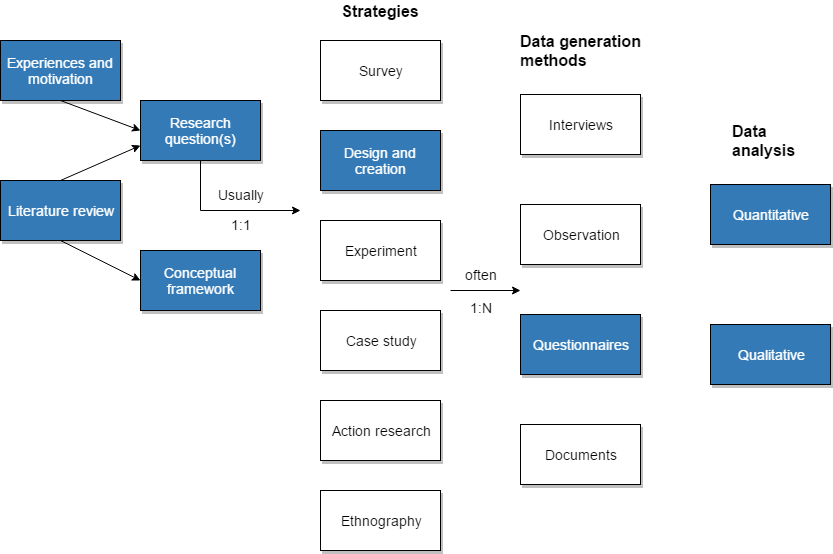
\includegraphics[width=0.8\textwidth]{fig/research_process.png}
    \caption{The outlined research process}
    \label{fig:research_process}
\end{figure}

Based on the motivation for doing this research, as well as the conducted literature review, the set of research questions were formed. These questions will be answered with the following strategy.

\section{Research Strategy}

This research requires the design and creation of a computer based artefact (Utsida) as a tool to answer the described research questions. However, the research strategy which will yield the desired results is considered a survey. Thus, the designated research strategy will be a combination of design and creation, and survey. 

\subsection{Design and Creation}

Utsida is the cornerstone of this research, as well as the required tool to answer RQ1. It will incorporate the AI methodology CBR to create a new way of reccommending relevant universities and courses for a student applying for an exchange program, and serve as a united place for required and handy data and information. 

It is of great importance that this system is well functioning and easy to use, if RQ1 is to be answered. Therefore, the the design and creation research strategy has to be followed. The system will be designed, created, and tested by relevant students, while the results of these tests will be carefully analyzed.

\subsubsection{Usability Testing}

To ensure sufficient usability and functionality for Utsida, there will be conducted waves of usability testing on carefully selected participants, mainly students who have a decent understanding of the current system for applying for an exchange program. Both technical competent- and less technical competent students will be tested.

These tests will help finding flaws in both general functionality and design, so that the system is as reliable as possible before finally conducting remote tests.

\subsubsection{System Testing of the CBR Module}

To answer RQ2, and thus to either confirm or reject the hypothesis that CBR is a feasible methodology to use in this problem domain, an experiment will be conducted in addition to any feedback recieved from the usability testing on the CBR retrieval process. Two CBR models; one without weighted attributes, and one with fully configured and modelled attributes will perform retrieval processes simultaneously, and the results will be analyzed. If the configured option, which will be used in this research, yields substantially more desired results, both in terms of correct retrieval, and the most relevance for the user, it is considered a success.

\subsection{Survey}

To answer RQ1, a survey will be conducted. First, a baseline will be established regarding students’ motivation and attitude towards applying for an exchange program at NTNU. This baseline will be created by utilizing a questionnaire which will be sent to a target group of students. These students will then be asked to try Utsida, followed by a new questionnaire which will establish whether the developed system had any substantial positive effect on these students.

The survey strategy will also be used to gain information of how to properly model the CBR module of Utsida. Each attribute in the model has to be weighted with proper importance, which require the average opinion of a large number of students to get as correct as possible. In this questionnaire, the students will be asked what they think are the most important aspects when selecting a geographical location, and a university for their exchange program.


\section{Data Generation Methods}

\subsection{Questionnaires}

All questionnaires which will be sent out in this research will be self-administrated, which promotes the opportunity to collect data from a large number of students at once. Because a student's thoughts of what is important, easy or convenient is rather subjective, as well as their attitude to the current system for applying for an exchange program, it is important to receive a large amount of data on this topic.

The recipients of the questionnaire should be students who have some experience with exchange studies. To acquire a larger group target group who fits this criteria, it is therefore desired to arrange a collaboration with NTNU's International Section, which regularly sends out surveys with to these students for various reasons.


\subsection{Interviews and Observation}
As a mean to acquire the needed information from the test subjects whom performed the usability tests, both observation and interviews were done. Each test was thoroughly observed, to see how the test subjects thought, and how they used the system, while each test ended with an interview. These data generation methods were used to improve the system to an acceptable state before performing remote testing and questionnaires.

\section{Data Analyzis}

The questionnaires which will be conducted will produce qualitative e data which will be analyzed in a statistical manner. It is considered a successful research if the latter questionnaire yields substantial improved results than the initial. 

\cleardoublepage